\newpage
\section{Empirical evaluation of Naive Bayes and Tree Augmented Naive Bayes}
\label{sec:eval}

I ran Naive Bayes and TAN on the Chess (King-Rook vs. King-Pawn) End Game Data Set \cite{chessEndGame}. The properties of the dataset are described below

$\bullet$ Number of Instances: 3196 

$\bullet$ Number of Attributes: 36 (all categorical)

$\bullet$ Classes (2):  -- White-can-win ("won") and White-cannot-win ("nowin").

$\bullet$ Class Distribution:
    In 1669 of the positions (52\%), White can win.
    In 1527 of the positions (48\%), White cannot win.

$\bullet$ The format for instances in this database is a sequence of 37 attribute values.
Each instance is a board-descriptions for this chess endgame.  The first
36 attributes describe the board.  The last (37th) attribute is the
classification: "win" or "nowin".  There are 0 missing values.
A typical board-description is

f,f,f,f,f,f,f,f,f,f,f,f,l,f,n,f,f,t,f,f,f,f,f,f,f,t,f,f,f,f,f,f,f,t,t,n,won

The names of the features do not appear in the board-descriptions.
Instead, each feature corresponds to a particular position in the
feature-value list.  For example, the head of this list is the value
for the feature "bkblk".  The following is the list of features, in
the order in which their values appear in the feature-value list:


[bkblk,bknwy,bkon8,bkona,bkspr,bkxbq,bkxcr,bkxwp,blxwp,bxqsq,cntxt,dsopp,dwipd,
 hdchk,katri,mulch,qxmsq,r2ar8,reskd,reskr,rimmx,rkxwp,rxmsq,simpl,skach,skewr,
 skrxp,spcop,stlmt,thrsk,wkcti,wkna8,wknck,wkovl,wkpos,wtoeg]
 
$\bullet$ Training set size used : 2130 instances. Number of $wons$ are  1109
number of $no$ $wins$ are  1021.


$\bullet$ Testing set size used : 1066 instances. Number of $wons$ are  560
number of $no$ $wins$ are  506.

$\bullet$ 35 of the 36 attributes are boolean the parameters of which have a $Beta(2,2)$ Prior and one attribute (number 15) is multinomial with 3 values which has a Dirichlet Prior(2,2,2) over it. The same prior is used for both Naive Bayes and for TAN. 
\begin{table}[h!]
\centering

\begin{tabular}{| m{3cm}| m{2cm} | m{2cm} |} 
\hline
  & Naive Bayes & TAN\\ 
\hline
 Test Set Accuracy & 87.05 \% & 93.34\%\\ 
\hline

\end{tabular}
\label{table:results}
\caption{Comparison between Naive Bayes and Tree Augmented Naive Bayes}
\end{table}


FIgure \ref{table:results} shows the comparison between Naive Bayes and Tree Augmented Naive Bayes.

The Bayes Net learnt from the dataset is shown in the Figure \ref{fig:bnn}. The number is the attribute number in the dataset its possible values are also shown. (Image has been rotated in order to fit on the page and read the attributes numbers clearly)

\begin{figure}[H]
	%\vspace{-0.4cm}
	\centering
	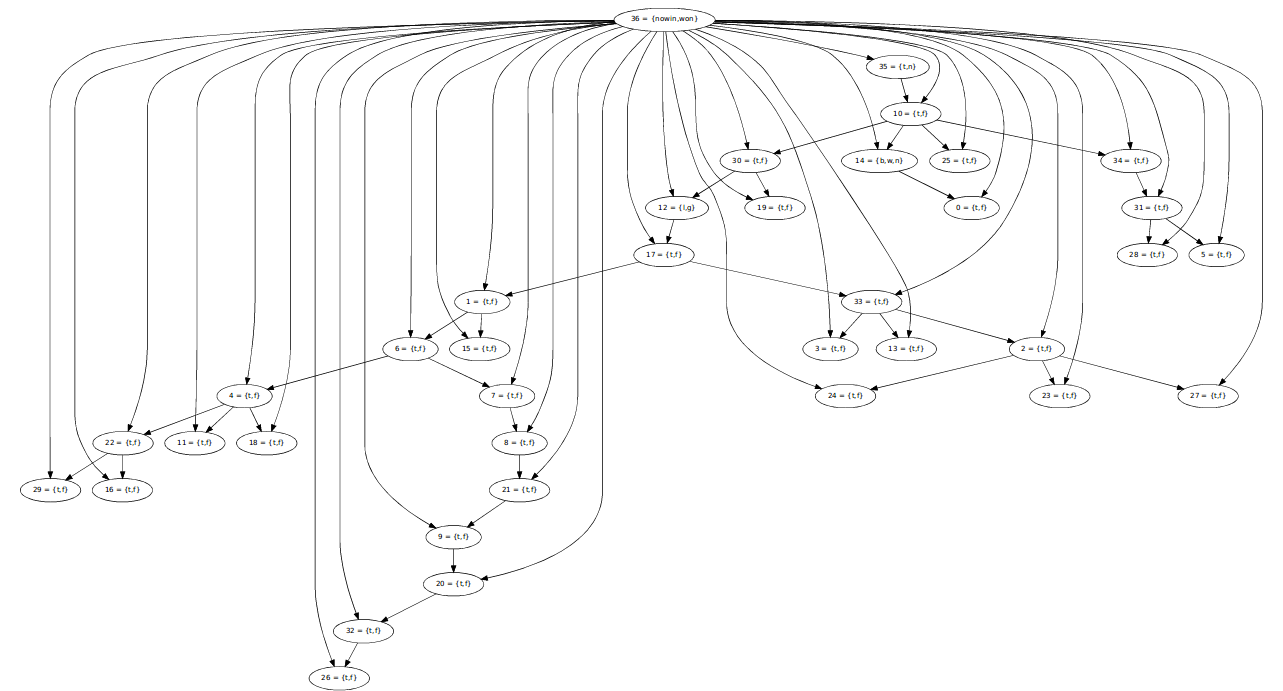
\includegraphics[angle=270,width=0.8\linewidth]{sections/imgs/evaluation/bn.png}
	\caption{Tree Augmented Bayes Net}
	\label{fig:bnn}
	%\vspace{-1.6cm}
\end{figure}